\documentclass[11pt,letterpaper]{article}
\usepackage[top=3cm, bottom=2cm, left=2cm, right=2cm, columnsep=20pt]{geometry}
\usepackage{pdfpages}
\usepackage{graphicx}
\usepackage{etoolbox}
\apptocmd{\sloppy}{\hbadness 10000\relax}{}{}
% \usepackage[numbers]{natbib}
\usepackage[T1]{fontenc}
\usepackage{ragged2e}
\usepackage[french]{babel}
\usepackage{listings}
\usepackage{color}
\usepackage{soul}
\usepackage[utf8]{inputenc}
\usepackage[export]{adjustbox}
\usepackage{caption}
\usepackage{amsmath}
\usepackage{amssymb}
\usepackage{float}
\usepackage{csquotes}
\usepackage{fancyhdr}
\usepackage{wallpaper}
\usepackage{siunitx}
\usepackage[indent]{parskip}
\usepackage{textcomp}
\usepackage{gensymb}
\usepackage{multirow}
\usepackage[hidelinks]{hyperref}
\usepackage{abstract}
\renewcommand{\abstractnamefont}{\normalfont\bfseries}
\renewcommand{\abstracttextfont}{\normalfont\itshape}
\usepackage{titlesec}
\titleformat{\section}{\large\bfseries}{\thesection}{1em}{}
\titleformat{\subsection}{\normalsize\bfseries}{\thesubsection}{1em}{}
\titleformat{\subsubsection}{\normalsize\bfseries}{\thesubsubsection}{1em}{}

\usepackage{xcolor}
\definecolor{codegreen}{rgb}{0,0.6,0}
\definecolor{codegray}{rgb}{0.5,0.5,0.5}
\definecolor{codepurple}{rgb}{0.58,0,0.82}
\definecolor{backcolour}{rgb}{0.95,0.95,0.92}
\lstdefinestyle{mystyle}{
    backgroundcolor=\color{backcolour},   
    commentstyle=\color{codegreen},
    keywordstyle=\color{magenta},
    numberstyle=\tiny\color{codegray},
    stringstyle=\color{codepurple},
    basicstyle=\ttfamily\footnotesize,
    breakatwhitespace=false,         
    breaklines=true,                 
    captionpos=b,                    
    keepspaces=true,                 
    numbers=left,                    
    numbersep=5pt,                  
    showspaces=false,                
    showstringspaces=false,
    showtabs=false,                  
    tabsize=2
}
\lstset{style=mystyle}

\usepackage[most]{tcolorbox}
\newtcolorbox{note}[1][]{
  enhanced jigsaw,
  borderline west={2pt}{0pt}{black},
  sharp corners,
  boxrule=0pt, 
  fonttitle={\large\bfseries},
  coltitle={black},
  title={Note:\ },
  attach title to upper,
  #1
}

%----------------------------------------------------

\setlength{\parindent}{0pt}
\DeclareCaptionLabelFormat{mycaptionlabel}{#1 #2}
\captionsetup[figure]{labelsep=colon}
\captionsetup{labelformat=mycaptionlabel}
\captionsetup[figure]{name={Figure }}
\newcommand{\inlinecode}{\normalfont\texttt}
\usepackage{enumitem}
\setlist[itemize]{label=\textbullet}

\begin{document}
\begin{titlepage}
\center

\begin{figure}
    \ThisULCornerWallPaper{.4}{Polytechnique_signature-RGB-gauche_FR.png}
\end{figure}
\vspace*{2 cm}

\textsc{\Large \textbf{PHS2223 --} Introduction à l'optique moderne}\\[0.5cm]
\large{\textbf{Équipe : 04}}\\[1.5cm]

\rule{\linewidth}{0.5mm} \\[0.5cm]
\Large{\textbf{Expérience 2}} \\[0.2cm]
\text{Objectif de caméra}\\
\rule{\linewidth}{0.2mm} \\[2.3cm]

\large{\textbf{Présenté à}\\
  Guillaume Sheehy\\
  Esmat Zamani\\[2.5cm]
  \textbf{Par :}\\
  Émile \textbf{Guertin-Picard} (2208363)\\
  Laura-Li \textbf{Gilbert} (2204234)\\
  Tom \textbf{Dessauvages} (2133573)\\[3cm]}

\large{\today\\
Département de Génie Physique\\
Polytechnique Montréal\\}

\end{titlepage}

%----------------------------------------------------

\tableofcontents
\pagenumbering{roman}
\newpage

\pagestyle{fancy}
\setlength{\headheight}{14pt}
\renewcommand{\headrulewidth}{0pt}
\fancyfoot[R]{\thepage}

\pagestyle{fancy}
\fancyhf{}
\renewcommand{\headrulewidth}{1pt}
\fancyhead[L]{\textbf{PHS2223}}
\fancyhead[C]{Rapport préliminaire}
\fancyhead[R]{\today}
\fancyfoot[R]{\thepage}

\pagenumbering{arabic}
\setcounter{page}{1}

%----------------------------------------------------

\section{Introduction}

Les objectifs de caméras modernes sont des systèmes physiques complexes, permettant de définir l'identité d'une image et dépendent par conséquent de la façon dont l'observateur veut représenter l'objet d'intérêt. Dans le cas le plus simple possible, cas d'étude de ce laboratoire, ces objectifs sont constitués de trois lentilles. Une fixe permettant de former une image nette et deux mobiles, utiles à l'ajustement de paramètres d'observations. Le premier de ces paramètres est lié au grossissement de l'objet observé. Pour prendre un clicher ou filmer une image lointaine, il faudra par exemple opter pour un téléobjectif à fort grossissement, ce qui n'est pas le cas lorsque le but est de faire un portrait rapproché. Cependant, décoller un portrait de l'arrière plan permet souvent de le mettre en valeur en le faisant ressortir. Ce flou recherché derrière l'objet observé est lié au deuxième paramètre étudié, que l'on appelle : profondeur de champ. Elle détermine le facteur de netteté associée à un éloignement vis-à-vis du point focal. Une grande profondeur de champ permettra donc de détailler l'arrière plan tandis qu'une faible profondeur de champ le floutera. Un dernier paramètre, davantage lié au système optique complet de l'objectif et de la mise en relation de ses éléments, nommé vignettage, définit l'assombrissement des bords de l'image en raison de l'ouverture d'arrêt. Le but de ce laboratoire est donc de caractériser un objectif de caméra simple, composé de trois lentilles. Les attentes sont de se familiariser et comprendre l'impact des paramètres d'observation de l'objectif sur une image enregistrée, tout en continuant de développer des habilités liée à l'alignement de systèmes optiques. Le présent rapport, présente la préparation à ce laboratoire, de la compréhension théorique du système étudié, à la méthodologie prévue pour ses manipulations ainsi que les hypothèses émises quant à leurs résultats. 

\section{Théorie}

\subsection{Système de caméra}

La figure \ref{schema_syst}, tirée de l'énoncé du laboratoire \textcolor{red}{Source A}, présente
l'intérieur du système de caméra sous forme de schéma des lentilles :

\begin{figure}[H]
  \centering
  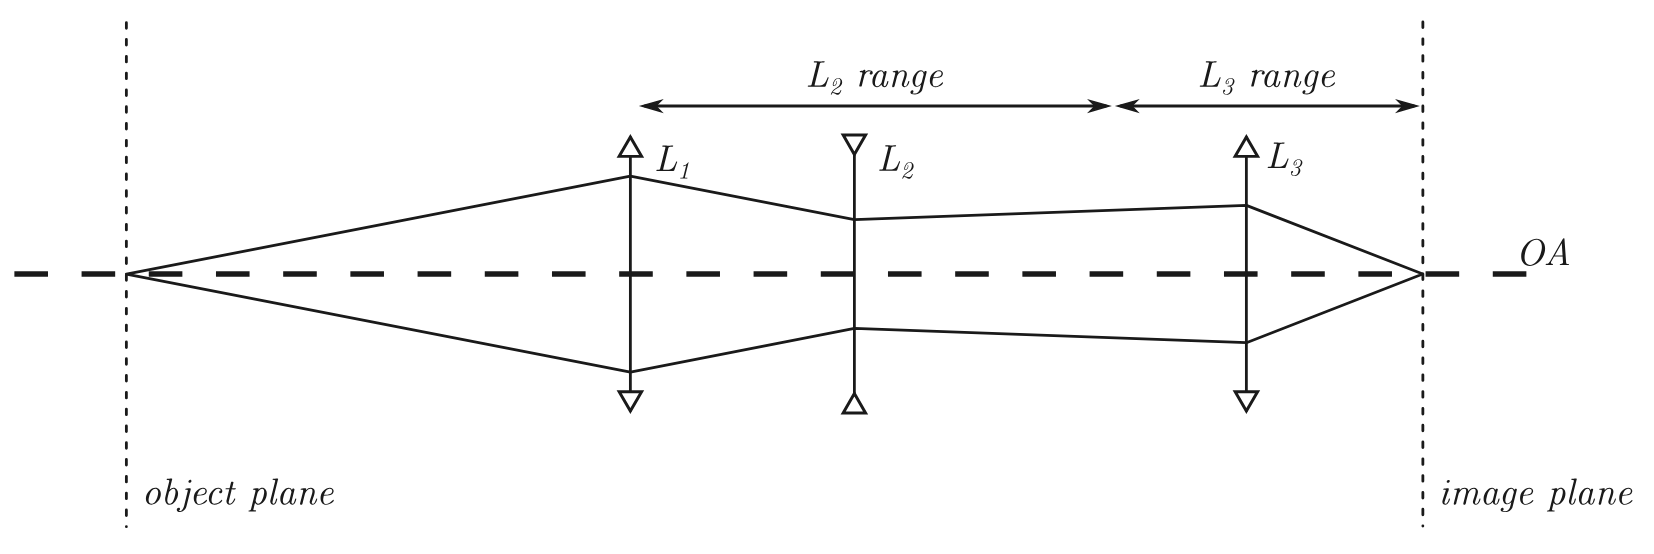
\includegraphics[scale=0.1]{systeme_optique.png}
  \caption{Schéma du système optique d'objectif de caméra à zoom et focus ajustable}
  \label{schema_syst}
\end{figure}

% Source A : énoncé du lab

\subsubsection{Grossissement}
Le grossissement correspond à l'augmentation apparente de la taille d'un objet lorsque celui-ci est observé à travers un système optique. En termes techniques, il s'agit d'un rapport entre la taille apparente de l'image et celle réelle \textcolor{red}{(Source B)}.

% Source B : https://uel.unisciel.fr/physique/optigeo/optigeo_ch17/co/apprendre_ch17_04.html#:~:text=Le%20grossissement%20est%20un%20nombre,distance%20minimale%20de%20vision%20distincte.

\subsubsection{Profondeur de champ}
La profondeur de champ décrit la distance autour du plan de mise au point avec laquelle les objets apparaissent suffisamment nets. En d'autres termes, ce concept optique réfère à la distance entre les points les plus rapprochés et ceux les plus éloignés du sujet qui sont reproduits avec une netteté acceptable dans une image \textcolor{red}{(Source 1)}. Appliquée à plusieurs sytèmes optiques tels que les caméras et les microscopes, cette notion de profondeur est influencée par les paramètres suivants : la distance focale, l'ouverture de l'objectif, et la distance de l'objet \textcolor{red}{(Source 2)}. 

% Source 1 : https://www.edmundoptics.fr/knowledge-center/application-notes/imaging/depth-of-field-and-depth-of-focus/#:~:text=La%20DOF%20d'un%20objectif,de%20mise%20au%20point%20optimale.

% Source 2 : Notes de cours L7_s4.pdf

\subsection{Modélisation mathématique par matrice de transfert}

\section{Méthodologie}

La méthode utilisée pour ce laboratoire vise à caractériser un objectif de caméra simple, composé de trois lentilles. La figure \ref{montage} présente sous la forme d'un schéma et d'une photographie, le montage utilisé, ainsi que son système optique. 

\begin{figure}[H]
  \centering
  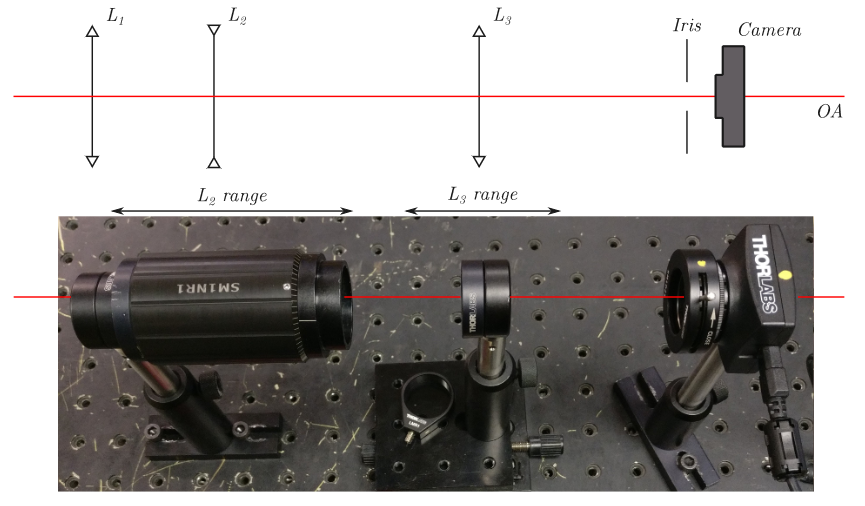
\includegraphics[scale=0.78]{Montage laboratoire 2.png}
  \caption{Schéma du système optique (en haut) du montage (en bas) utilisé pour le laboratoire.}
  \label{montage}
\end{figure}

Le matériel utilisé pour ce montage étant : 

\begin{itemize}
    \item Lentille $L_1 = 150 mm$, $\phi_1 = 25.4 mm$
    \item Lentille $L_2 = -75 mm$, $\phi_1 = 25.4 mm$
    \item Lentille $L_3 = 75 mm$, $\phi_1 = 25.4 mm$
    \item Iris ajustable SM1D25
    \item Tube à lentille ajustable 75 mm (\textit{zoom housing}) SM1NR1
    \item Plateforme de translation > 25 mm
    \item Caméra USB Thorlabs DDC1645C
    \item Pièces optomécaniques nécessaires (BA1, PH2, PH3, TR2, TR3, LMR1, ...)
\end{itemize}

La première étape consiste à aligner le montage, en utilisant des iris d'alignement et en maximisant le focus sur la caméra. Il faudra ensuite, pour chaque paramètre établir une série de mesures en fonction de la variable d'intérêt. La liste des clichés à prendre est : 

\begin{itemize}
    \item La profondeur de champ à 1 m (2 positions extrêmes du zoom)
    \item La résolution à 1 m (2 positions extrêmes du zoom)
    \item Mesure du vignetting à 1 m et à $\infty$ (2 positions extrêmes du zoom)
    \item Image d’objet à l’infini (2 positions extrêmes du zoom)
\end{itemize}

Dans tous les cas, les clichés seront à prendre en double, pour chacune des valeurs extrêmes de zoom. La lentille $L_2$ sera donc toujours placée aux extrémités de sa plage de déplacement. Pour ce qui est de $L_3$, elle sera positionnée de sorte que l'objet d'intérêt soit toujours au focus. L'objet imagé sera positionné en fonction du paramètre à mesurer. A un mètre pour le grossissement, la résolution et à un mètre puis l'infini pour le vignetting. Dans le cas de la profondeur de champ, puisqu'elle nécessite de mesurer une plage de valeur, l'objet sera positionné à un mètre de l'objectif, puis avancé et ensuite reculé jusqu'à sortir du plan focal, afin de déterminer la distance entre les valeurs d'avancement et d'éloignement maximum.

\section{Hypothèses}

% TODO : code en annexe

Afin de pouvoir prédire les phénomènes qui pourront être observés en laboratoire, un
programme Python disponible en annexe a été développé afin de résoudre analytiquement
le système par la méthode des matrices. Ce programme commence tout d'abord par construire
la matrice de transfert du système, puis il paramétrise l'écart entre les lentilles selon
la position de $L_2$ par rapport à $L_1$. Enfin, il calcule les différentes caractéristiques
qui suivent.

\subsection{Profondeur de champ}

Premièrement, le programme calcule la profondeur de champ en fonction de la position de
la lentille $L_2$. Le résultat est présenté à la figure \ref{prof_champ_plot}.

\begin{figure}[H]
  \centering
  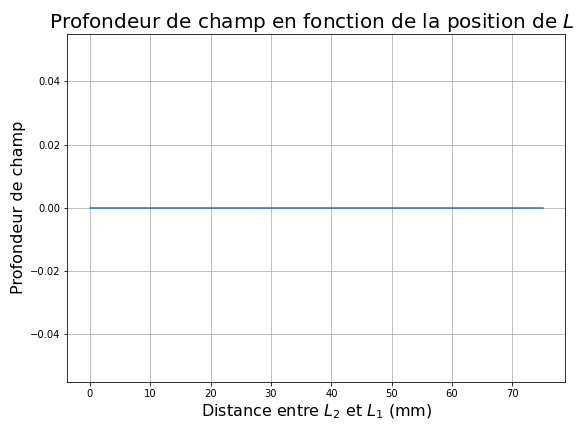
\includegraphics[scale=0.55]{prof_champ.png}
  \caption{Graphique de la profondeur de champ en fonction de la position de la lentille 
  $L_2$ suite au calcul de Python}
  \label{prof_champ_plot}
\end{figure}

Ainsi, il est possible de faire comme hypothèse que la profondeur du champ n'est pas affectée
par la position de $L_2$.

\subsection{Résolution}

Ensuite, la figure \ref{gross_plot} montre le grossissement de l'image en fonction de la
position de $L_2$.

\begin{figure}[H]
  \centering
  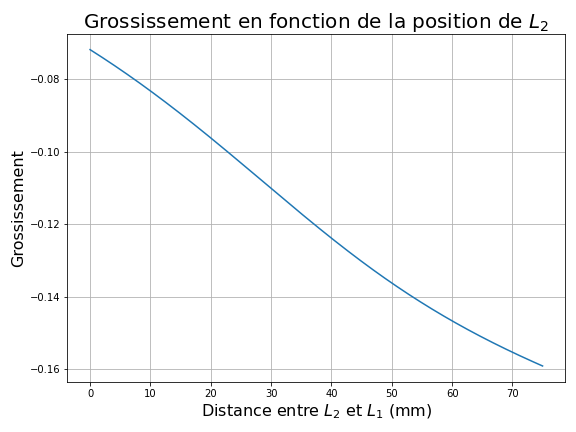
\includegraphics[scale=0.55]{grossissement.png}
  \caption{Graphique du grossissement d'une image en fonction de la position de la lentille
  $L_2$ suite au calcul de Python.}
  \label{gross_plot}
\end{figure}

Découlant directement de ce résultat, il est possible de visualiser la résolution en fonction
de la position de la lentille, tel que montré à la figure \ref{res_plot}. Cela montre la taille
d'un pixel de la caméra (\textit{pixel pitch}), qui vaut 3.6 micromètres pour la caméra THORLABS, dans le plan objet \textcolor{red}{Source B}.

% Source B : https://www.thorlabs.com/catalogpages/obsolete/2020/DCC1645C.pdf

\begin{figure}[H]
  \centering
  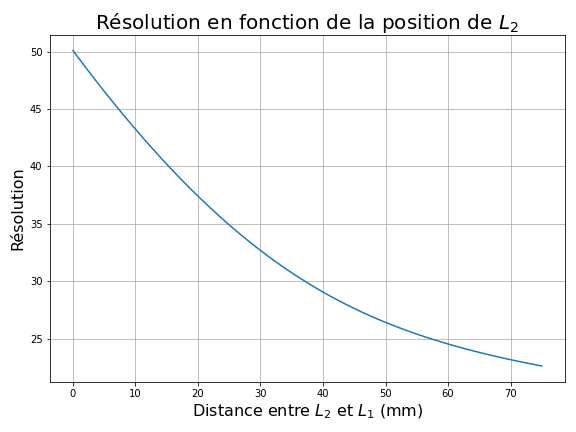
\includegraphics[scale=0.55]{Resolution.png}
  \caption{Graphique de la résolution de la caméra en fonction de la position de la lentille
  $L_2$ suite au calcul de Python.}
  \label{res_plot}
\end{figure}

Ainsi, il est possible de prédire que le grossissement (qui est inversé en raison du signe 
négatif) augmente plus la distance entre $L_2$ et $L_1$ augmente. Sans surprise, une relation 
réciproque est prédite pour la résolution, qui décroît plus cette distance augmente.

\subsection{Facteur de zoom}

Enfin, selon la figure \ref{gross_plot}, il est possible de prendre les deux extrêmes de la courbe 
pour trouver une prédiction dufacteur de zoom. Calculé par le programme, le résultat est un facteur
d'environ 0.45.
\clearpage

% \bibliographystyle{unsrtnat}
% \bibliography{My_Library}

\end{document}
